\documentclass[a4paper,12pt]{article}

% Packages
\usepackage{amsmath, amssymb, amsthm}
\usepackage{amsfonts} % For using math fonts
\usepackage{graphicx} % For including images
\usepackage{geometry} % For page layout
\usepackage{hyperref} % For hyperlinks
\usepackage{tcolorbox}
\usepackage{color}
\usepackage{xcolor}
\usepackage{tikz-feynman}
\usepackage{float} 
\usepackage{listings}
\usepackage{transparent}
\usepackage{enumitem}

\usepackage{feynmp-auto} % For Feynman diagrams


\lstset{ 
  language=Python,                 % choose the language of the code
  basicstyle=\ttfamily\footnotesize, % set the font to typewriter (monospace)
  numbers=left,                    % display line numbers
  keywordstyle=\color{blue}\bfseries,      % Color and bold for keywords
  commentstyle=\color{gray},              % Color for comments
  stringstyle=\color{red},                 % Color for strings
  identifierstyle=\color{black},           % Color for identifiers
  numberstyle=\tiny\color{gray},    % set the style of line numbers
  stepnumber=1,                    % step between two line numbers
  numbersep=5pt,                   % distance of line numbers from the code
  backgroundcolor=\color{white},   % set background color
  showspaces=false,                % don't show spaces as underscores
  showstringspaces=false,          % don't emphasize spaces in strings
  showtabs=false,                  % don't show tabs
  frame=single,                    % add a frame around the code
  tabsize=2,                       % set default tab size
  captionpos=b,                    % set caption position to bottom
  breaklines=true,                 % automatic line breaking
  breakatwhitespace=false,         % break lines at whitespace
  escapeinside={\%*}{*)},          % if you want to add LaTeX inside the code
}

\newcommand{\hrulewithspace}{\vspace{10pt}\hrule\vspace{10pt}}


\usepackage{titling}   




\usepackage{titlesec}

% Section formatting
\titleformat{\section}
  {\normalfont\large\bfseries} % Common formatting for both numbered and unnumbered
  {\ifnum\value{section}>0 \thesection \else \fi} % Display section number if it's numbered, otherwise nothing
  {0.5em}
  {\ifnum\value{section}>0 \raggedright \else \centering \fi} % Left align if numbered, center if unnumbered
  []


% Page layout
\geometry{
    margin=1in
}


\begin{document}
\begin{titlepage}
    \begin{center}
        \vspace*{2cm}
        
 % University name
        {\Large Example 2 for /r/LLMPhysics} \\[1.5cm]
        
        % Top horizontal line
        \hrule
        \vspace{1cm}
        
        % Title
        {\Huge \textbf{Analyzing Collider Events}} \\[1cm]
        
        % Bottom horizontal line
        \hrule
        \vspace{1.5cm}
         \Large {Conquest{\transparent{0.1}\(\bigstar\)}Ace}\\ [1 cm]
        % Additional Information
 

         % Logo
         {\transparent{0.05}
\includegraphics[width=0.25\textwidth]{logo.png} \\[1cm]}

        % Date (Optional)
        % {\large \today}


        \vfill

    \end{center}
\end{titlepage}

\section*{Simulating Two Body Decays}
When an energetic beam of protons collides with a target material, it produces lots of particles, many of which are pions. We want to simulate the decay of $\pi^0 \to \gamma \gamma $.
\section{Theory}
We need to consider the relativistic kinematics and some quantum field theory. 

Our neutral pion is a short-lived meson composed of a quantum superposition of up-antiup ($u \bar{u}$) and down-antidown ($d \bar{d}$) quarks. 

\[
\pi^0 = \frac{1}{\sqrt{2}} (u \bar{u} - d \bar{d})
\]
It decays via the \textbf{electromagnetic interaction} into two photons:

\[ \pi^0 \to \gamma \gamma  \] 

\subsection{Conservation Laws of $\pi^0$ at rest}
\begin{itemize}[label=$\triangleright$]
\item  Energy needs to be conserved: $E_{initial} = E_{final}$. The energy conservation of a pion at rest is then:
\begin{align*}
    E &= pc \\
    E_{\pi^0} &= m_{\pi^0} c^2 \\
    E_{\pi^0} = E_\gamma + E_\gamma &= \frac{m_{\pi^0} c^2}{2} + \frac{m_{\pi^0} c^2}{2} \\
    p_1 = p_2 &= \frac{m_{\pi^0} c}{2} 
\end{align*}

\item  momentum needs to be conserved: In the pion's rest frame, the total momentum of the decay products, must be zero. So the two photons are emitted in opposite directions with equal magnitudes of momentum: 
\begin{align*}
    \vec{p}_{\pi^0} = 0 = \vec{p}_1 + \vec{p}_2 &\implies \vec{p}_1 = -\vec{p}_2 \\
\end{align*}

\item  angular momentum needs to be conserved: pion has spin-0, so two photons must have angular momentum 0. Since photons have spin-1, their helicity is $\pm 1$ , so the spins must be opposite to cancel each other out. 
\item  parity needs to be conserved: Pion has negative parity, so the two photon system must match that.
\item  charge needs to be conserved: Photons are neutral, so charge is conserved.
\end{itemize}


\subsection{Kinematics of Two Body Decay}

In the rest frame of our pion, it has mass $m_{\pi^0} = 135 \text{ MeV}$ and no initial momentum. After decaying into the two photons, the photons travel at the speed of light, $c$ just in opposite directions of one another.

In general for a particle at rest $p^\mu =(mc, 0,0,0)$ with energy $E = mc^2$  decaying to two particles with momenta $p_1$ and $p_2$:
\begin{align*}
E &= E_1 + E_2 \\
mc^2 &= E_1 + E_2
\end{align*}
We can solve for the momenta using the energy-momentum relation: $E^2 = p^2c^2 + m^2c^4$ for each particle.
\begin{align*}
E_1^2 &= p_1^2c^2 + m_1^2c^4 \\
E_2^2 &= p_2^2c^2 + m_2^2c^4
\end{align*}
Squaring both sides and using energy conservation:
\begin{align*}
m^2c^4 = (E_1 + E_2)^2 = E_1^2 + E_2^2 + 2E_1E_2 \\
\end{align*}
Substituting $E_1^2$ and $E_2^2$:
\begin{align*}
m^2c^4 = p_1^2c^2 + m_1^2c^4 + p_2^2c^2 + m_2^2c^4 + 2E_1E_2
\end{align*}
And the following:
\begin{align*}
m^2c^4 - m_1^2 c^4 -m_2^2 c^4 = p_1^2c^2 + p_2^2c^2 + 2E_1E_2
\end{align*}
$p_1 = p_2 = p$
\begin{align*}
m^2c^4 - m_1^2 c^4 -m_2^2 c^4 = 2p^2c^2 + 2E_1E_2
\end{align*}
Now solve for $E_1E_2$:
\begin{align*}
E_1 E_2 = \frac{(m^2 +m_1^2 -m_2^2(m^2+m_2^2-m_1^2)}{4m^2}c^4
\end{align*}
Lastly we have the following for the magnitude of the momentum of the daughter particles of the decay:
\begin{align*}
p = \frac{\sqrt{(m^2 - (m_1 + m_2)^2)(m^2 - (m_1 - m_2)^2)}}{2m}c
\end{align*}



\noindent When the pion is not at rest, i.e has momentum  $p_{\pi^0}$, we can first analyze the decay in the rest frame of the pion like we did just have, then apply a Lorentz boost to the decay products to the lab frame.

Suppose pion has an initial 4-momenta: $p^\mu = (\gamma mc, \gamma vm, 0, 0)$ where $\gamma = \frac{1}{\sqrt{1-v^2}}$. Then, the decay products must be Lorentz-boosted to the lab frame. 
\begin{align*}
E' = \gamma(E - vp_x) \\
p_x' = \gamma(p_x + vE) \\
\end{align*}

\subsection{Decay Rates}
The decay $\pi^0 \to \gamma \gamma $ is given by:
\[
    \Gamma_{\pi \rightarrow \gamma\gamma} = \frac{(2\pi)^4}{2E_\pi} \int |M_{\pi \rightarrow \gamma\gamma}|^2 \delta(E_\pi - E_{\gamma1} - E_{\gamma2}) \delta^3(\mathbf{p}_\pi - \mathbf{p}_{\gamma1} - \mathbf{p}_{\gamma2}) \frac{d^3\mathbf{p}_{\gamma1}}{(2\pi)^3 2E_{\gamma1}} \frac{d^3\mathbf{p}_{\gamma2}}{(2\pi)^3 2E_{\gamma2}}
\]


For this we need the matrix element, which we can get my analyzing the interaction of the specific coupling of the pion to photons. After we have that, we will need to perform the integration to get the total decay rate. This means we will need to know our detector's acceptance and other experimental constraints. 

The neutral pion is composed of up and down quarks: $\pi^0 = \frac{1}{\sqrt{2}} (u \bar{u}- d \bar{d})$. We get an effective Lagrangian for the pion-photon interaction:
\[
\mathcal{L}_{\pi^0 \gamma \gamma} =  \frac{\alpha}{8\pi f_{\pi}} \pi^0 F_{\mu \nu} \bar{F}^{\mu \nu}
\]
From this alongside with the Feynman rules, we can calculate the decay width:
\[
\Gamma(\pi^0 \rightarrow \gamma \gamma) = \frac{\alpha^2 m_{\pi^0}}{64 \pi^3 f_{\pi}^2} \approx 7.8 \text{ eV}
\]
The branching ratio is:
\[
\text{BR}(\pi^0 \rightarrow \gamma \gamma) = \frac{\Gamma(\pi^0 \rightarrow \gamma \gamma)}{\Gamma_{\text{total}}} \approx 98.8\%
\]
In our simulation we are only considering this decay mode, and ignoring the other decays such as the Dalitz  decay ($\pi^0 \rightarrow e^+ e^- \gamma$) for example. 


\section{Lorentz product, invariant masses, and Lorentz Transformation}

\subsection{Lorentz product}
The Lorentz product/Minkowski inner product of two four-vectors $A^\mu$and $B^\mu$ is:
\[
A \cdot B = A^\mu B_\mu = A^0 B^0 - \vec{A} \cdot \vec{B} = A^0 B^0 - A^1 B^1 - A^2 B^2 - A^3 B^3
\]

\begin{lstlisting}
def lorentz_product(A, B):
    """Computes the Lorentz product of two four-vectors."""
    return A[0] * B[0] - np.dot(A[1:], B[1:])
\end{lstlisting}


\noindent To test the Lorentz product, we can use some known properties and simple cases:

  1. Self-product gives squared invariant mass:
    \[
    P \cdot P = m^2
    \]
\begin{lstlisting}
#testing the functions
P = np.array([5, 3, 4, 0])  # E = 5, p = (3,4,0)
expected_mass_squared = 5**2 - (3**2 + 4**2)  # Should be 0 (massless case)
computed_mass_squared = lorentz_product(P, P)
print(computed_mass_squared, expected_mass_squared, expected_mass_squared-computed_mass_squared)
assert np.isclose(computed_mass_squared, expected_mass_squared), "Invariant mass test failed!"
\end{lstlisting}
Output:
    \begin{lstlisting}
        0 0 0
    \end{lstlisting}

2. We can also check if two orthogonal four-vectors $A^\mu$ and $B^\mu$ have a Lorentz product of zero:
    \[
    A \cdot B = 0
    \]
\begin{lstlisting}
A = np.array([2, 1, 1, 0])
B = np.array([1, 1, -1, 0])  # Manually chosen so that their Lorentz product is 0
assert np.isclose(lorentz_product(A, B), 0), "Orthogonality test failed!"
\end{lstlisting}
Output:
    \begin{lstlisting}
        0 0 0
    \end{lstlisting}

and lastly, can check that the Lorentz product remains unchanged after a Lorentz boost:
\begin{lstlisting}
P = np.array([10, 3, 4, 0])
velocity = np.array([0.6, 0, 0])  # Boost along x-direction
P_boosted = lorentz_transform(P, velocity)
print(lorentz_product(P, P), lorentz_product(P_boosted, P_boosted))
assert np.isclose(lorentz_product(P, P), lorentz_product(P_boosted, P_boosted)), "Lorentz invariance test failed!"
\end{lstlisting}
Output:
    \begin{lstlisting}
        75 75.0
    \end{lstlisting}
So, the functions are all behaving like we expect them to. We can then say, this product is invariant under Lorentz transformations meaning it has the same value in all inertial frames of references. 

\subsection{Invariant mass}
The invariant mass of a particle with four-momentum vector $P^\mu= E, \vec{P}$ is defined as:
\begin{align*}
m^2c^2 &= P \cdot P = P^\mu P_\mu = P^0 P^0 - \vec{P} \cdot \vec{P} = E^2 - \vec{P}^2 \\
m^2 c^2 &= E^2 - \vec{p} \cdot \vec{p} 
\end{align*}
and with $c=1$:
\(
m^2 = E^2 - \vec{p} \cdot \vec{p}
\)

\noindent For a pair of particles with four-momentum vectors $P_1^\mu$ and $P_2^\mu$, with system mass $M$:
\begin{align*}
M^2 &= (P_1 + P_2)^2 = (P_1 + P_2) \cdot (P_1 + P_2) \\
M^2 &= P_1 \cdot P_1 + P_2 \cdot P_2 + 2P_1 \cdot P_2 \\
M^2 &= m_1^2 + m_2^2 + 2P_1 \cdot P_2
\end{align*}
where $m_1$ and $m_2$ are the invariant masses of the two particles.

The code for the invariant mass and system mass:
\begin{lstlisting}
def invariant_mass(P):
    """Computes the invariant mass of a four-momentum vector P."""
    return np.sqrt(P[0]**2 - np.dot(P[1:], P[1:]))

def system_mass(P1, P2):
    """Computes the invariant mass of a system of two particles."""
    P_total = P1 + P2
    return np.sqrt(lorentz_product(P_total, P_total))
\end{lstlisting}

\begin{lstlisting}
def test_invariant_mass():
    P = np.array([5, 3, 4, 0])
    expected_mass = np.sqrt(5**2 - (3**2 + 4**2))
    assert np.isclose(invariant_mass(P), expected_mass), "Invariant mass test failed!"
\end{lstlisting}

Output: 
\begin{lstlisting}
Invariant mass test passed!
\end{lstlisting}

\subsection{Lorentz Transformation}
The Lorentz transformation matrix for a boost in an arbitrary direction \( \mathbf{v} = (v_x, v_y, v_z) \) is given by:

\[
\Lambda^\mu_{\ \nu} = 
\begin{pmatrix}
\gamma & -\gamma \beta n_x & -\gamma \beta n_y & -\gamma \beta n_z \\
-\gamma \beta n_x & 1 + (\gamma - 1) n_x^2 & (\gamma - 1) n_x n_y & (\gamma - 1) n_x n_z \\
-\gamma \beta n_y & (\gamma - 1) n_y n_x & 1 + (\gamma - 1) n_y^2 & (\gamma - 1) n_y n_z \\
-\gamma \beta n_z & (\gamma - 1) n_z n_x & (\gamma - 1) n_z n_y & 1 + (\gamma - 1) n_z^2
\end{pmatrix}
\]

where \( \beta = \frac{v}{c} \), \( \gamma = \frac{1}{\sqrt{1 - \beta^2}} \), and \( \mathbf{n} = (n_x, n_y, n_z) = \frac{\mathbf{v}}{v} \).

The code for this is:
\begin{lstlisting}
def lorentz_transform(P, v):
    """Applies a Lorentz boost to a four-vector P in the direction of velocity v."""
    v = np.array(v)
    v_mag = np.linalg.norm(v)
    if v_mag == 0:
        return P  # No boost needed
    
    beta = v_mag / 1  # Assume c=1
    gamma = 1 / np.sqrt(1 - beta**2)
    n = v / v_mag  # Normalize direction
    
    # Lorentz transformation matrix
    Lambda = np.array([
        [gamma, -gamma * beta * n[0], -gamma * beta * n[1], -gamma * beta * n[2]],
        [-gamma * beta * n[0], 1 + (gamma - 1) * n[0]**2, (gamma - 1) * n[0] * n[1], (gamma - 1) * n[0] * n[2]],
        [-gamma * beta * n[1], (gamma - 1) * n[1] * n[0], 1 + (gamma - 1) * n[1]**2, (gamma - 1) * n[1] * n[2]],
        [-gamma * beta * n[2], (gamma - 1) * n[2] * n[0], (gamma - 1) * n[2] * n[1], 1 + (gamma - 1) * n[2]**2]
    ])
    
    return np.dot(Lambda, P)
\end{lstlisting}

\noindent We have already verified the Lorentz transform using our Lorentz product. So we can just refer to that for the check of this function.

\section{Two Body Decay of a particle of mass $M$ at rest}
When a particle of mass $M$ decays into two particles with mass $m_1$ and $m_2$, the total energy and momentum must be conserved. In the rest frame of the parent particle, the total energy before the decay is $M$ and the total momentum before decay is $0$ . As we discussed before, the decay products will move in opposite directions with equal and opposite momenta. 

Using the energy-momentum relation: $E^2-p^2=m^2$, we can find the energy and momentum of the decay products. 
\[
E_1 = \frac{M^2 + m_1^2 - m_2^2}{2M}, \quad E_2 = \frac{M^2 + m_2^2 - m_1^2}{2M}
\]
The magnitude of the momenta are then:
\[
p = \sqrt{E_1^2 - m_1^2} = \sqrt{E_2^2 - m_2^2}
\]
To ensure we get an isotropic decay (equal probability in all directions), we can sample the polar angle $\theta$ from a uniform distribution in $\cos\theta = 2\text{rand}()-1$ (this gives us values from [-1,1]) and the azimuthal angle $\phi$ uniformly from $0$ to $2\pi$.

Then we convert to cartesian coordinates:
\[
p_x = p \sin\theta \cos\phi, \quad p_y = p \sin\theta \sin\phi, \quad p_z = p \cos\theta
\]
These are the momenta of the decay product of the first particle and the second particle is simply the negative of the first.

\begin{lstlisting}
def two_body_decay(M, m1, m2):
    """Generates two random four-momenta for a two-body decay in the rest frame of the decaying particle."""
    E1 = (M**2 + m1**2 - m2**2) / (2 * M)
    E2 = (M**2 + m2**2 - m1**2) / (2 * M)
    p_mag = np.sqrt(E1**2 - m1**2)  # Magnitude of the momentum
    
    # Generate a random isotropic direction
    theta = np.arccos(2 * np.random.rand() - 1)  # Uniform in cos(theta)
    phi = 2 * np.pi * np.random.rand()  # Uniform in phi
    
    p1 = np.array([E1, p_mag * np.sin(theta) * np.cos(phi), p_mag * np.sin(theta) * np.sin(phi), p_mag * np.cos(theta)])
    p2 = np.array([E2, -p1[1], -p1[2], -p1[3]])  # Opposite direction
    
    return p1, p2
\end{lstlisting}

We did not need to know the matrix element to compute the kinematics of the two-body decay because we are dealing with conservation laws and relativistic constraints. This allows to get the momentum distribution. 

If we were to apply dynamics with the Lagrangian, we would need to find the matrix element. If we wanted to generate more correct physics-based events, we would need to consider the actual probabilistic distribution of the decays rather than assuming our events are uniform.

\section{Mass $M$ moving with velocity $v$}

After calculating the momentum of the daughter particles in the rest frame, we need to boost to the lab frame to each daughters four-momentum. 

\[
P^{'\mu} = \Lambda^\mu_nu P^\nu
\]

\begin{lstlisting}
def two_body_decay(M, m1, m2, v):
    """Generates two random four-momenta for a two-body decay in the rest frame of the decaying particle,
    then boosts them to the lab frame where the decaying particle moves with velocity v."""
    E1 = (M**2 + m1**2 - m2**2) / (2 * M)
    E2 = (M**2 + m2**2 - m1**2) / (2 * M)
    p_mag = np.sqrt(E1**2 - m1**2)  # Magnitude of the momentum
    
    # Generate a random isotropic direction
    theta = np.arccos(2 * np.random.rand() - 1)  # Uniform in cos(theta)
    phi = 2 * np.pi * np.random.rand()  # Uniform in phi
    
    p1 = np.array([E1, p_mag * np.sin(theta) * np.cos(phi), p_mag * np.sin(theta) * np.sin(phi), p_mag * np.cos(theta)])
    p2 = np.array([E2, -p1[1], -p1[2], -p1[3]])  # Opposite direction
    
    # Boost to the lab frame
    p1_lab = lorentz_transform(p1, v)
    p2_lab = lorentz_transform(p2, v)
    
    return p1_lab, p2_lab

\end{lstlisting}


\section*{Some Validation of the Decays}
We take some random 4-momenta decay the pion and check the conservation of energy and momentum of the products. 
\[
E_{\pi^0} = E_1 + E_2 \\
\vec{p}_{\pi^0} = \vec{p}_1 + \vec{p}_2
\]
To see how well these hold, compute the energy and momentum differences and plot their distributions:
\[
E_{\pi^0} - (E_1 + E_2) \\
|\vec{p}_{\pi^0} - (\vec{p}_1 + \vec{p}_2)|
\]

\begin{lstlisting}
# Conservation checks
df["energy_diff"] = df["E"] - (df["E1"] + df["E2"])
df["momentum_diff"] = np.sqrt(
    (df["px"] - (df["px1"] + df["px2"]))**2 +
    (df["py"] - (df["py1"] + df["py2"]))**2 +
    (df["pz"] - (df["pz1"] + df["pz2"]))**2
)

# Plot energy and momentum conservation
fig, axes = plt.subplots(1, 2, figsize=(12, 5))

axes[0].hist(df["energy_diff"], bins=100, color="blue", alpha=0.7)
axes[0].set_title("Energy Conservation: $E_{\pi^0} - (E_1 + E_2)$")
axes[0].set_xlabel("Energy Difference [GeV]")
axes[0].set_ylabel("Count")

axes[1].hist(df["momentum_diff"], bins=100, color="red", alpha=0.7)
axes[1].set_title("Momentum Conservation: $|\\vec{p}_{\pi^0} - (\\vec{p}_1 + \\vec{p}_2)|$")
axes[1].set_xlabel("Momentum Difference [GeV/c^2]")
axes[1].set_ylabel("Count")

plt.tight_layout()
plt.show()
\end{lstlisting}

\begin{figure}[H]
    \centering
    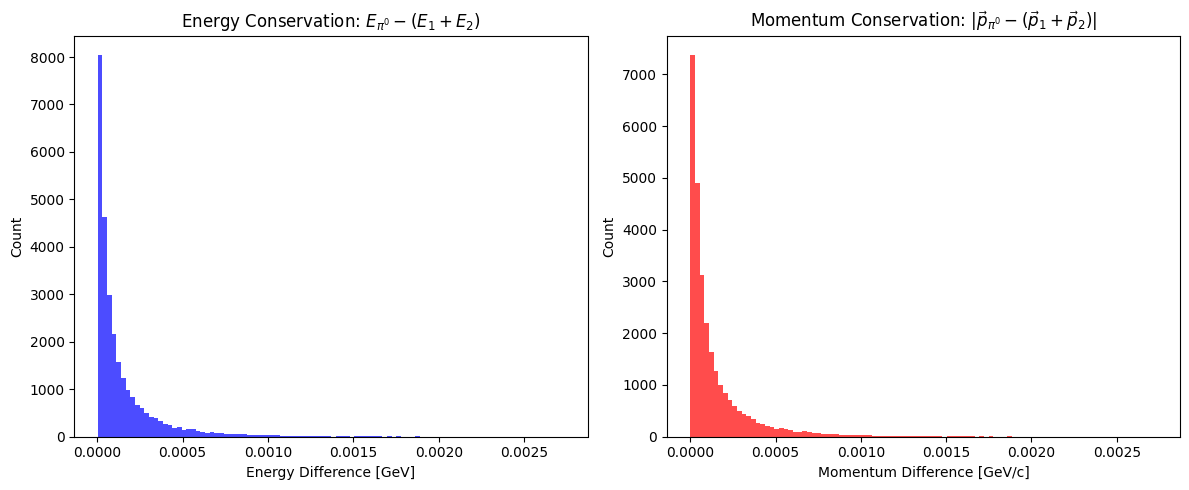
\includegraphics[width=0.8\textwidth]{SimulatingTwoBodyDecays/figures/energyconservation.png}
    \caption{Histograms showing the distribution of energy and momentum differences for the two-body decay.}
    \label{fig:energy_momentum_conservation}

\end{figure}

These graphs can be applied to both the decay of the particles at rest or in motion. The results are the same and we have conservation of energy and momentum (within the range of numerical precision). There is additional validation of almost all the functions and simulation in the code.

\section{Simulation of the Two-Body Decay, $\pi^0 \to \gamma \gamma $ }
The following is a simulation of the two-body decay. It is a vectorized version of the previous code so it can handle a large number of events efficiently. 
The key steps are:
\begin{enumerate}
    \item Initialization of variables and arrays
    \item For each $\pi^0$ in pi0\_momenta, perform a two-body decay to simulate the production of two photons using the two\_body\_decay function. We vectorized this function to handle a large number of events efficiently.
    \item Boost to Lab Frame using the vectorzed\_lorentz\_transform function
    \item Photon Check: an event is detected if at least one of the two photons hit the detector
    \item Calculate Fraction
\end{enumerate}

\begin{lstlisting}
def vectorized_lorentz_transform(p, v):
    """
    Perform a Lorentz boost on a batch of 4-vectors.
    
    Parameters
    ----------
    p : numpy.ndarray
        Array of 4-vectors in the rest frame, shape (N, 4), with columns [E, px, py, pz].
    v : numpy.ndarray
        Array of boost velocities, shape (N, 3). (Assuming units where c=1.)
    
    Returns
    -------
    numpy.ndarray
        Boosted 4-vectors in the lab frame, shape (N, 4).
    """
    # Compute beta^2 for each event (v^2)
    beta2 = np.sum(v**2, axis=1, keepdims=True)  # shape: (N,1)
    # Calculate gamma factor for each event
    gamma = 1.0 / np.sqrt(1.0 - beta2)             # shape: (N,1)
    # Dot product between the spatial momentum and the boost velocity
    bp = np.sum(p[:, 1:] * v, axis=1, keepdims=True)  # shape: (N,1)
    
    # Calculate the factor (gamma - 1)/beta2 safely. Set to 0 when beta2 is nearly zero.
    with np.errstate(divide='ignore', invalid='ignore'):
        gamma2 = np.where(beta2 > 1e-12, (gamma - 1.0) / beta2, 0.0)  # shape: (N,1)
    
    # Boost the spatial components:
    # p[:, 1:] is (N,3) and v is (N,3); the operations are elementwise.
    spatial = p[:, 1:] + gamma2 * bp * v + gamma * p[:, :1] * v  # shape: (N,3)
    # Boost the energy component:
    energy = gamma * (p[:, :1] + bp)  # shape: (N,1)
    
    # Concatenate boosted energy and spatial parts along axis 1.
    boosted = np.hstack([energy, spatial])
    return boosted

def estimate_detection_fraction_vectorized(pi0_momenta, M, detector_size=1.0, distance=10.0):
    """
    Estimate the fraction of \pi^0 decays for which at least one photon hits the detector.
    
    The detector is assumed to be a square centered at (x, y) = (0, 0) in a plane 
    located at z = distance. The size of the detector is detector_size (length of a side).
    
    Parameters
    ----------
    pi0_momenta : numpy.ndarray
        Lab frame 4-momenta of the \pi^0 particles (shape: [N,4] with columns [E, px, py, pz]).
    M : float
        Mass of the \pi^0 particle (in GeV/c^2).
    detector_size : float, optional
        Size of the detector (side length), by default 1.0.
    distance : float, optional
        z-distance to the detector plane, by default 10.0.
    
    Returns
    -------
    float
        The estimated geometric efficiency (fraction of decays detected).
    """
    n_decays = len(pi0_momenta)
    
    # Generate random angles for isotropic decays in the pion rest frame.
    cos_theta = 2 * np.random.rand(n_decays) - 1
    theta = np.arccos(cos_theta)
    phi = 2 * np.pi * np.random.rand(n_decays)
    
    # In the rest frame of the \pi^0, energy = |p| for a photon. Each photon gets half the mass.
    p_mag = M / 2.0

    # Photon 1 in the rest frame: 4-vector [E, px, py, pz]
    p1_rest = np.column_stack([
        np.full(n_decays, p_mag),                # Energy
        p_mag * np.sin(theta) * np.cos(phi),
        p_mag * np.sin(theta) * np.sin(phi),
        p_mag * cos_theta
    ])
    
    # Photon 2 has exactly the opposite momentum.
    p2_rest = np.column_stack([
        np.full(n_decays, p_mag),                # Energy
        -p_mag * np.sin(theta) * np.cos(phi),
        -p_mag * np.sin(theta) * np.sin(phi),
        -p_mag * cos_theta
    ])
    
    # Compute the boost velocity of the \pi^0: v = p/E
    # pi0_momenta has columns [E, px, py, pz]
    v = pi0_momenta[:, 1:] / pi0_momenta[:, :1]  # shape: (N,3)
    
    # Boost both photons to the lab frame.
    p1_lab = vectorized_lorentz_transform(p1_rest, v)
    p2_lab = vectorized_lorentz_transform(p2_rest, v)
    
    def check_hits(p):
        """
        Check if the boosted photon (p) hits the detector.
        
        p is expected to be a numpy array of shape (N,4) for lab-frame 4-vectors.
        """
        # We are interested in the photon's z-component; if it is nearly zero or negative (moving backward), it won't hit.
        pz = p[:, 3]
        nonzero = np.abs(pz) > 1e-8
        # For photons moving toward the detector (i.e. pz > 0), compute the parametric distance t such that z = distance.
        # For non-moving or backward-moving photons, set t = infinity.
        t = np.where((pz > 0) & nonzero, distance / pz, np.inf)
        # The photon hits at positions (x_hit, y_hit)
        x_hit = p[:, 1] * t
        y_hit = p[:, 2] * t
        # Check if (x_hit, y_hit) fall within half the detector size.
        hit = (np.abs(x_hit) <= detector_size / 2.0) & (np.abs(y_hit) <= detector_size / 2.0)
        # Only count if the photon is moving forward.
        hit = hit & (pz > 0)
        return hit
    
    hits1 = check_hits(p1_lab)
    hits2 = check_hits(p2_lab)
    
    # An event is detected if at least one of the two photons hits the detector.
    detected = hits1 | hits2
    fraction_detected = np.mean(detected)
    return fraction_detected
\end{lstlisting}

Here we apply the functions defined above for our 120 GeV momenta array. 
\begin{lstlisting}
if __name__ == '__main__':
    # Define the \pi^0 mass (in GeV/c^2)
    M_pi0 = 0.1349768
    n_events = 100000  # Number of decays to simulate
    
    # Generate random lab frame \pi^0 momenta.
    # We'll sample the spatial momentum components from a normal distribution.
    lab_momenta_spatial = np.random.normal(0, 1, (n_events, 3))
    # Compute the energy using E = sqrt(p^2 + m^2)
    energies = np.sqrt(np.sum(lab_momenta_spatial**2, axis=1) + M_pi0**2)
    # Construct the \pi^0 momenta array with columns [E, px, py, pz]
    pi0_momenta = np.column_stack([energies, lab_momenta_spatial])
    
    # Estimate the geometric efficiency:
    fraction = estimate_detection_fraction_vectorized(momenta_array, M_pi0,
                                                      detector_size=1.0,
                                                      distance=10.0)
    print(f"Geometric efficiency: {fraction:.6f}")
    print(f"Expected number of detected events: {fraction * n_events:.0f}")
\end{lstlisting}
We get outputs of around 0.36 or 36\%. 

We also apply the functions for a isotropic distribution of momenta and get a similar result of 0.16\%

\begin{lstlisting}
if __name__ == '__main__':
    # Define the \pi^0 mass (in GeV/c^2)
    M_pi0 = 0.1349768
    n_events = 100000  # Number of decays to simulate
    
    # Generate random lab frame \pi^0 momenta.
    # We'll sample the spatial momentum components from a normal distribution.
    lab_momenta_spatial = np.random.normal(0, 1, (n_events, 3))
    # Compute the energy using E = sqrt(p^2 + m^2)
    energies = np.sqrt(np.sum(lab_momenta_spatial**2, axis=1) + M_pi0**2)
    # Construct the \pi^0 momenta array with columns [E, px, py, pz]
    pi0_momenta = np.column_stack([energies, lab_momenta_spatial])
    
    # Estimate the geometric efficiency:
    fraction = estimate_detection_fraction_vectorized(pi0_momenta, M_pi0,
                                                      detector_size=1.0,
                                                      distance=10.0)
    print(f"Geometric efficiency: {fraction:.6f}")
    print(f"Expected number of detected events: {fraction * n_events:.0f}")
\end{lstlisting}

\subsection{Changing the detector coverage}

The probability a photon hits the detector is determined by:
\[
P_{\text{hit} \approx \frac{\text{Detector Area}}{4\pi \times (\text{Distance})^2}}
\]
Our original setup had a detector of  $1\,m \times 1\,m$ at $10\,m $ which had a solid angle $\Delta \Omega = \frac{1}{10^2} = 0.01\,sr$ the total solid angle is then $4\pi \approx 12.566\,sr$ This gives us a probability per photon of : 
\[
\frac{0.01}{12.566} \approx 0.000796 \,(0.08\%)
\]
\begin{itemize}[label=$\triangleright$]
    \item Probability for 2 photons: 
\[
1 - (1 - 0.000796)^2 \approx 0.00159 \,(0.16\%)
\]
\end{itemize}
\textbf{Effect of Detector Size}

1. Smaller Detector (e.g., $0.1\,m \times 0.1\,m$):
\begin{itemize}[label=$\triangleright$]
    \item Area: \(0.01\,m^2 \to \Delta \Omega = \frac{0.01}{100} = 0.0001\) sr
    \item Probability per photon: 
   \(
   \frac{0.0001}{12.566} \approx 8 \times 10^{-6}
   \)
    \item Expected fraction: 
   \(
   \approx 1.6 \times 10^{-5} \,(0.0016\%)
   \)
\end{itemize}
2. Larger Detector (e.g., $10\,m \times 10\,m$):
\begin{itemize}[label=$\triangleright$]
   \item Area: $100\,m^2 \to \Delta \Omega = \frac{100}{100} = 1\,sr$
   \item Probability per photon: \(
   \frac{1}{12.566} \approx 0.0796
   \)
   \item Expected fraction: 
   \(
   \approx 1 - (1 - 0.0796)^2 \approx 0.153 \,(15.3\%)
   \)
\end{itemize}

\subsection{Simulation Results}
To estimate the geometric acceptance, also known as geometric efficiency, of a hypothetical detector for detecting photons resulting from the decay of neutral pions $ (\pi^0 \to \gamma \gamma )$. The detector is positioned 10 meters downstream from the target, featuring a 1m x 1m front face.

\subsubsection*{Simulation Setup}

The simulation was conducted using a vectorized process to model the two-body decay of $\pi^0$ particles into two photons. Initially, the momenta of the $\pi^0$ were sourced from a dataset simulating proton-target collisions. These momenta were used as inputs to model the decay events in the rest frame of the $\pi^0$ particles.

\subsubsection*{Lorentz Boost to the Lab frame}

Photons arising from these decays were subject to relativistic transformations, as each photon pair was translated from the $\pi^0$  rest frame to the lab frame using Lorentz boosts. A vectorized method was employed for the transformations, allowing efficient computation across the entire dataset.

\subsubsection*{Detection Criteria}

For each photon, its trajectory was assessed to determine whether it intersected with the detector's plane at $z=10m$. An intersection was counted as a 'hit' if the coordinates at intersection remained within the $[-0.5m,0.5m]$ bounds of the detector face in both x and y dimensions.

The fraction of decays wherein at least one photon intersected with the detector plane defines the geometric acceptance. Across the simulations, the geometric efficiency was calculated as follows:

\begin{equation*}
    \text{Geometric Efficiency} = \frac{\text{Number of Hits}}{\text{Total Number of Decays}}
\end{equation*}

\subsubsection*{Results and Interpretation}
The simulation resulted with varying output due to random chance. In the table below, are the results of the geometric efficiency for different outputs with random seeds.

 

\begin{table}[H]
    \centering
    \begin{tabular}{|c|c|}
        \hline
        \textbf{Geometric Efficiency} \\
        \hline
        0.367154 \\
        0.366336 \\
        0.367865 \\
        \hline
    \end{tabular}
    \caption{Geometric Efficiency for 120 GeV decays provided by the data file}
    \label{tab:geometric_efficiency}
\end{table}

\begin{table}[H]
    \centering
    \begin{tabular}{|c|c|}
        \hline
        \textbf{Geometric Efficiency} \\
        \hline
        0.001670 \\
        0.001480 \\
        0.001540 \\
        \hline
    \end{tabular}
    \caption{Geometric Efficiency for Isotropic Decays}
    \label{tab:geometric_efficiency}
\end{table}

When using random isotropic decays, we find the geometric efficiency to be approximately 0.0016. This aligns with the theoretical prediction of 0.16\%.


However, when using the data file provided, which came from $\pi^0$ with average momenta of 120 GeV, we find the geometric efficiency to be approximately 0.367. This is significantly higher than the theoretical prediction of 0.16\%. This discrepancy is likely due to the fact that the data file provided is not isotropic, and thus the geometric efficiency is higher.

We can see that the data is not isotropic by simply seeing that the average energy of the photons is 6 GeV and has maximum energy of 108 GeV. 

\begin{lstlisting}
print(E.mean())
print(E.max())
\end{lstlisting}
output
\begin{lstlisting}
6.031258107431741
108.53296975773868
\end{lstlisting}
compared to 
\begin{lstlisting}
1.602811772293395
5.149393972687484
\end{lstlisting}
of the isotropic data
\begin{figure}[H]
    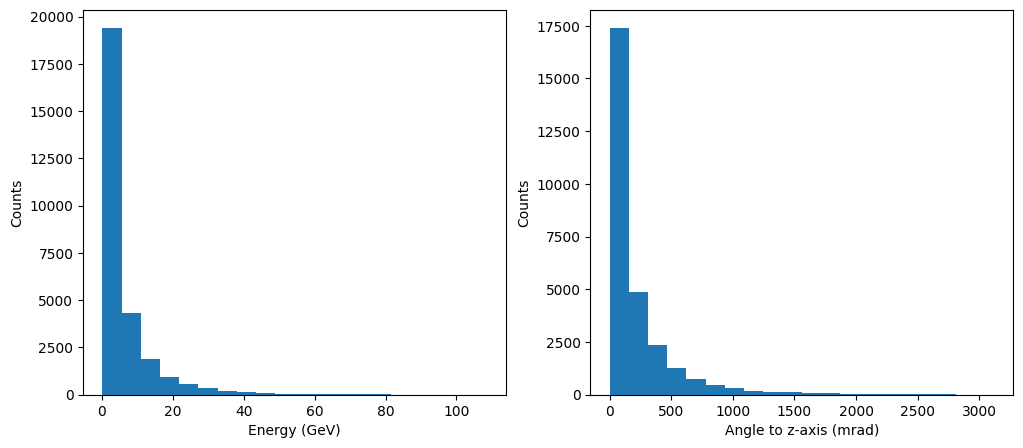
\includegraphics[width=\textwidth]{SimulatingTwoBodyDecays/figures/120distri.png}
    \caption{Distribution of the 120 GeV Decay}
    \label{fig:GeometricEfficiency}
\end{figure}

\begin{figure}[H]
    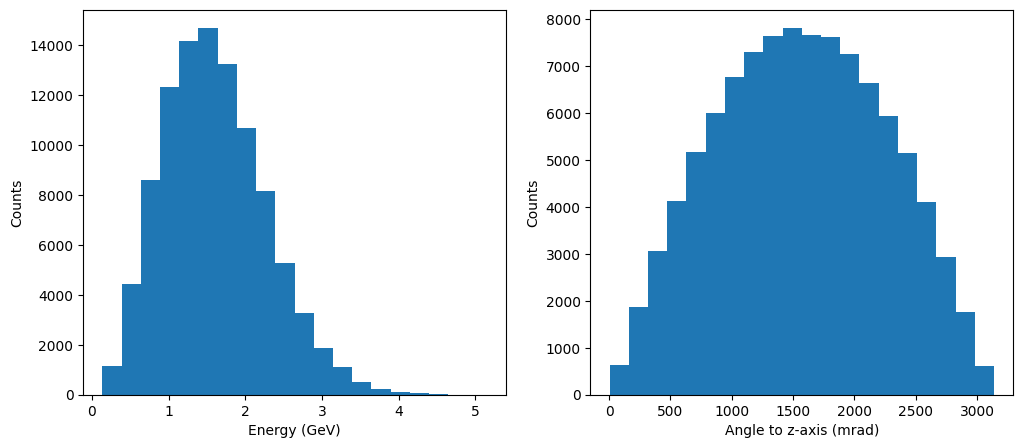
\includegraphics[width=\textwidth]{SimulatingTwoBodyDecays/figures/isodistri.png}
    \caption{Distribution of the Isotropic Decay}
    \label{fig:GeometricEfficiency}
\end{figure}

It is clear that the initial momenta and angles of the $\pi^0$ particles significantly influenced the likelihood of detection, demonstrating the sensitivity of geometric acceptance to the kinematic conditions of particle decays. 

\subsection{Changing Detector Sizes}
\begin{lstlisting}
results = []
configurations = [
    {"detector_size": 10.0, "distance": 1.0},
    {"detector_size": 10.0, "distance": 10.0},
    {"detector_size": 10.0, "distance": 100.0},
    {"detector_size": 0.1, "distance": 1.0},
    {"detector_size": 0.1, "distance": 10.0},
    {"detector_size": 0.1, "distance": 100.0},
]

for config in configurations:
    detector_size = config["detector_size"]
    distance = config["distance"]
    fraction = estimate_detection_fraction_vectorized(pi0_momenta, M_pi0,
                                                        detector_size=detector_size,
                                                        distance=distance)
    results.append({
        "detector_size": f"{detector_size:.1f}m x {detector_size:.1f}m",
        "distance": f"{distance:.1f}m",
        "efficiency": f"{fraction:.6f}"
    })

# Display results in a nice table
print("| Detector Size      | Distance | Geometric Efficiency |")
print("|----------------------|----------|----------------------|")
for result in results:
    print(f"| {result['detector_size']:<20} | {result['distance']:<8} | {result['efficiency']:<20} |")
\end{lstlisting}

\begin{table}[h!]
    \centering
    \begin{tabular}{|l|c|c|}
        \hline
        Detector Size & Distance (m) & Geometric Efficiency \\
        \hline
        1.0m x 1.0m & 10.0 & 0.369180980831 \\
        10.0m x 10.0m & 1.0 & 0.991713787830 \\
        10.0m x 10.0m & 10.0 & 0.912016785803 \\
        10.0m x 10.0m & 100.0 & 0.370852448522 \\
        0.1m x 0.1m & 1.0 & 0.368398591700 \\
        0.1m x 0.1m & 10.0 & 0.021551264270 \\
        0.1m x 0.1m & 100.0 & 0.000284505139 \\
        \hline
    \end{tabular}
    \caption{Geometric Efficiency for Different Detector Configurations}
    \label{tab:geometric_efficiency}
\end{table}

and for the isotropic data:

\begin{table}[h!]
    \centering
    \begin{tabular}{|l|c|c|}
        \hline
        Detector Size & Distance (m) & Geometric Efficiency \\
        \hline
        1.0m x 1.0m & 10.0 & 0.001630000000 \\
        10.0m x 10.0m & 1.0 & 0.458140000000 \\
        10.0m x 10.0m & 10.0 & 0.086440000000 \\
        10.0m x 10.0m & 100.0 & 0.001460000000 \\
        0.1m x 0.1m & 1.0 & 0.001510000000 \\
        0.1m x 0.1m & 10.0 & 0.000010000000 \\
        0.1m x 0.1m & 100.0 & 0.000000000000 \\
        \hline
    \end{tabular}
    \caption{Geometric Efficiency for Different Detector Configurations}
    \label{tab:geometric_efficiency}
\end{table}


%bibliography
\newpage
\nocite{*}
\bibliographystyle{plain} % or use plain, alpha, ieeetr, etc.
\bibliography{references}

\end{document}

